% ============================================================== 1. Introduction
\section{Introduction}
\label{sec:intro}

Deep learning classifiers for dermoscopy images can match dermatologists on curated test sets
\cite{esteva2017dermatologist}, but their performance can drop on
data that differ from the training distribution \cite{daneshjou2022disparities}, and robust models need
large and diverse training data that are held by separate institutions. Privacy regulation and
institutional policy often prevent pooling such data, which has made federated learning (FL), in which
sites train a shared model without exchanging images, a central approach for multi-institutional medical
imaging \cite{rieke2020future,sheller2020federated,dayan2021exam}. Claims about FL
for clinical use, however, rest on benchmarks, and a benchmark is informative only if its evaluation
reflects the situation of a new lesion at a participating or a new site.

For skin lesions, Fed-ISIC2019, the dermoscopy benchmark of the FLamby suite \cite{flamby2022}, is
widely used. Its six clients correspond to acquisition sources of the ISIC 2019 challenge data
\cite{codella2018isic,tschandl2018ham,combalia2019bcn} and differ in size, class mix and imaging
device. Federated and personalized methods are compared on its fixed split, and the reported differences
between them are often a few points of balanced accuracy \cite{flamby2022,tavakoli2024fendafl}.

The benchmark split assigns individual images rather than lesions to the training and test sets. Many
lesions in the underlying collections were photographed several times, for example at follow-up visits or
with different magnifications. An image-level split therefore places correlated views of one lesion on
both sides (Figure~\ref{fig:leakage}a), so the test set partly measures recognition of lesions seen in
training rather than diagnosis of new ones. Such leakage is a known cause of over-optimistic results in
machine learning \cite{kapoor2023leakage,varoquaux2022failures}. In dermatology, duplicates and
problematic partitions have been documented in centralized datasets
\cite{cassidy2022isic,groger2023reliable,abhishek2025dermamnist}, and subject-level splitting has
inflated accuracy in histopathology and brain MRI \cite{bussola2021tiles,yagis2021leakage}. We found no
study that quantifies lesion-level leakage per client in Fed-ISIC2019 or examines its consequences for
federated method comparisons, calibration and conformal coverage. Because clients differ in size and
acquisition protocol, leakage need not be uniform: in the official Fed-ISIC2019 split, 93\% of one
client's test images have a sibling image in training, compared with 0.1\% in another. Leakage may
therefore distort not only absolute accuracy but also comparisons between methods that fit client-level
data to different degrees, such as local and personalized models.

A second gap concerns reliability at the level of the individual site. FL studies usually report a
single accuracy over the pooled test set, whereas a clinician needs calibrated probabilities
\cite{guo2017calibration} and, ideally, prediction sets whose error rate is controlled at their own
site. Conformal prediction provides sets with distribution-free marginal coverage under exchangeability
\cite{vovk2005algorithmic,angelopoulos2023gentle}, and federated variants target coverage on the
mixture of clients, under label shift, or for personalized and group-defined targets
\cite{lu2023fcp,humbert2023oneshot,plassier2023labelshift,min2025pfcp,wen2026gcfcp}. A
threshold computed from pooled scores can under-cover individual clients while meeting its mixture
target, and a threshold computed from a small client's own data controls coverage on average but varies
strongly between calibration samples. How these effects play out on the Fed-ISIC2019 clients, how they
interact with leakage and with the repeated images of one lesion, and how they change on unseen clients
or images from another device has, to our knowledge, not been reported.

In this study we audit federated skin lesion classification on Fed-ISIC2019 with image-level and
lesion-grouped splits. We train up to eight federated, personalized, centralized and local methods with
three encoder configurations (a fully fine-tuned convolutional network, the same network frozen, and a
frozen dermatology foundation model) and evaluate accuracy, method rankings, calibration and conformal
coverage overall and per client, on held-out clients and on smartphone images. Confirmatory analyses
followed a version-controlled protocol fixed before the corresponding runs, and we report the tests that
failed alongside those that succeeded. Our contributions are:
\begin{enumerate}
  \item A per-client audit of lesion-level leakage in Fed-ISIC2019, of the apparent accuracy gain it
    produces, and of its consequences for method rankings, calibration and conformal coverage, together
    with a randomized sibling-exposure experiment that estimates the effect of leakage on fixed test
    images.
  \item Evidence that leakage inflates accuracy also with frozen encoders, including a dermatology
    foundation model, and randomized and capacity-matched experiments showing that its size grows with how
    closely a classifier fits its training lesions, not with personalization as such.
  \item A per-client analysis of federated conformal calibration that separates mixture from per-client
    coverage and accounts for repeated images of one lesion, and EB-ShrinkFCP, an empirical-Bayes
    shrinkage rule for per-client thresholds that met its pre-specified criterion for one of two encoders.
  \item Lesion-grouped splits, code, predictions and the complete protocol history, released to support
    leakage-free federated benchmarking.
\end{enumerate}

The remainder of the paper is organized as follows. Section~\ref{sec:related} reviews related work,
Section~\ref{sec:methods} describes the data, models and analyses, Section~\ref{sec:results} reports the
results by research question, Section~\ref{sec:discussion} discusses their implications and limitations,
and Section~\ref{sec:conclusion} concludes.

\begin{figure*}[!t]
  \centering
  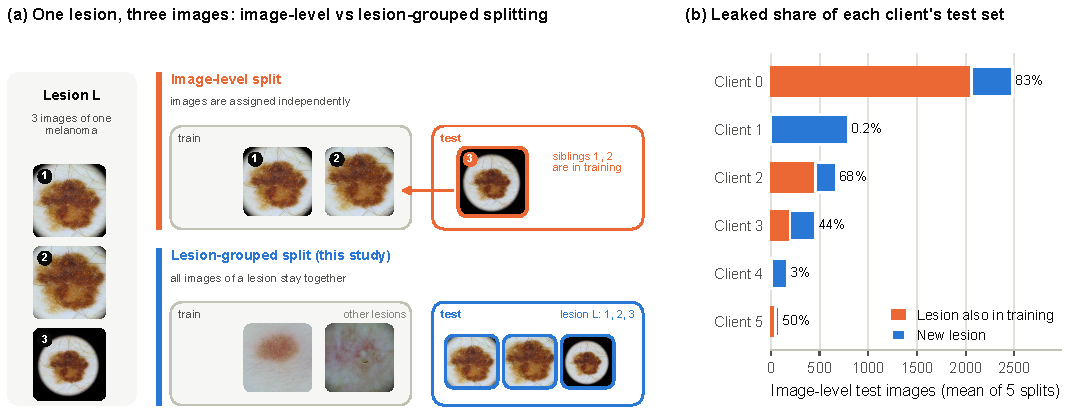
\includegraphics[width=\textwidth]{Fig1_design_leakage}
  \caption{Lesion-level leakage in Fed-ISIC2019. (a) The three images of one melanoma of client~0 (lesion
  BCN\_0000057; images ISIC\_0057997, ISIC\_0065360 and ISIC\_0068295, all sharing this identifier in the
  ISIC 2019 metadata). In the official FLamby split, the first two are training images and the third is a
  test image; under a lesion-grouped split, all images of a lesion stay on one side. (b) Image-level test
  images per client that are leaked (their lesion also has images in training) or new; percentages give
  the leakage rate as the mean over five image-level re-splits (the official split is reported in
  Table~\ref{tab:dataset}). Images: ISIC 2019 (CC-BY-NC 4.0).}
  \label{fig:leakage}
\end{figure*}
